\documentclass[a4paper,parskip,headheight=38pt]{scrartcl} % article or scrartcl
\usepackage[utf8]{inputenc}
\usepackage{amsmath,amssymb,amsfonts}
\usepackage[%
  automark,
  headsepline                %% Separation line below the header
]{scrlayer-scrpage}
\usepackage[english]{babel}
\usepackage{hyphenat}
\usepackage[hidelinks]{hyperref}
\usepackage[top=1.4in, bottom=1.5in, left=1in, right=1in]{geometry}
\usepackage{lastpage}
\usepackage{csquotes}
\usepackage{microtype}
\usepackage{datetime}

\usepackage[normalem]{ulem}
\usepackage{enumerate}
\usepackage{hyperref}

% \usepackage{multicol}
\usepackage{graphicx}
\usepackage{graphics}
% \usepackage{float}
% \usepackage{caption}

\setkomafont{pagehead}{\normalfont\sffamily\footnotesize}
\addtolength{\headheight}{+6pt}
\lohead{Ben Wiederhake, s9bewied@\ldots, 2541266}
\rohead{ES16, Set 1, Page {\thepage}/{\pageref*{LastPage}}}

\newtimeformat{mytime}{\twodigit{\THEHOUR}\twodigit{\THEMINUTE}\twodigit{\THESECOND}}
\settimeformat{mytime}
\newdateformat{mydate}{\twodigit{\THEYEAR}\twodigit{\THEMONTH}\twodigit{\THEDAY}}
\cfoot{\tiny\texttt{ID \mydate\today\currenttime}}
\chead{} % Needed because now the \subsections get displayed
\pagestyle{scrheadings}

% \renewcommand{\headrulewidth}{0pt}
% \addtolength{\textheight}{+30mm}
% \addtolength{\textwidth}{+50mm}
% \addtolength{\hoffset}{-7mm}

% \newcommand{\Omicron}{\ensuremath{\mathcal{O}}}
% \newcommand{\omicron}{\ensuremath{o}}
% \newcommand{\set}[1]{\{#1\}}
% \newcommand{\abs}[1]{\lvert #1 \rvert}

\begin{document}

\section*{Problem 1: Simulink}

\subsection*{Part 1: Sketch}

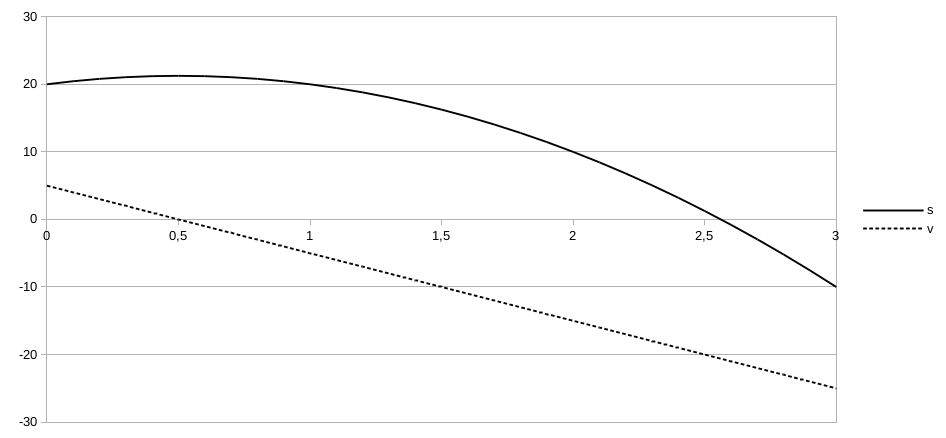
\includegraphics[width=\textwidth]{p1-sketch}
% I know, and I'm sorry.

\subsection*{Part 2: Differential equations}

\begin{align*}
    v(0) &= 5 \\
    dv/dt &= -10 \\
    s(0) &= 20 \\
    ds/dt &= v(t)
\end{align*}


\section*{Problem 2: Car Motion on a Slope}

FIXME


\section*{Problem 3: Stability of Equilibria}

FIXME


\section*{Problem 4: Cyclist}

FIXME


\section*{Problem 5: Oscillator}

FIXME


\section*{Problem 6: Geiger-Müller Counter}

FIXME


\end{document}
